\begin{figure}[t]
\centering
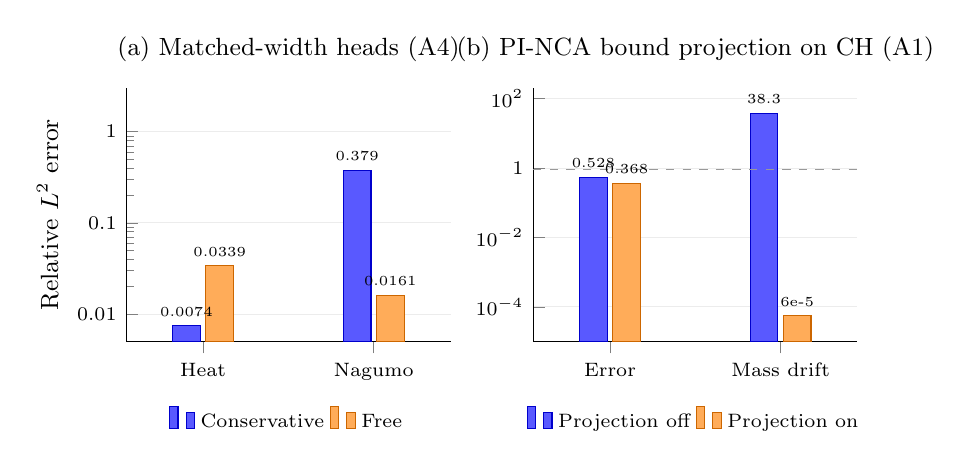
\begin{tikzpicture}
\begin{axis}[
    name=conservation,
    width=0.47\linewidth,height=4.8cm,
    ybar,bar width=10pt,
    ymode=log,log origin=infty,
    ymin=0.005,ymax=3,
    ylabel={Relative $L^2$ error},
    symbolic x coords={Heat,Nagumo},xtick=data,
    enlarge x limits=0.45,
    ytick={0.01,0.1,1},
    yticklabels={0.01,0.1,1},
    title={(a) Matched-width heads (A4)},
    title style={font=\small},
    tick label style={font=\scriptsize},
    label style={font=\small},
    nodes near coords,
    nodes near coords style={font=\tiny},
    point meta=explicit symbolic,
    legend style={font=\scriptsize,at={(0.5,-0.23)},anchor=north,draw=none},
    legend columns=2,
    axis lines*=left,
    ymajorgrids,grid style={gray!15}
]
\addplot[fill=blue!65,draw=blue!80!black] coordinates
  {(Heat,0.00743) [0.0074] (Nagumo,0.379) [0.379]};
\addplot[fill=orange!65,draw=orange!80!black] coordinates
  {(Heat,0.0339) [0.0339] (Nagumo,0.0161) [0.0161]};
\legend{Conservative,Free}
\end{axis}
\begin{axis}[
    at={(conservation.east)},anchor=west,xshift=1.05cm,
    width=0.47\linewidth,height=4.8cm,
    ybar,bar width=10pt,
    ymode=log,log origin=infty,
    ymin=1e-5,ymax=200,
    symbolic x coords={Error,Mass drift},xtick=data,
    enlarge x limits=0.45,
    ytick={1e-4,1e-2,1,100},
    yticklabels={$10^{-4}$,$10^{-2}$,$1$,$10^{2}$},
    title={(b) PI-NCA bound projection on CH (A1)},
    title style={font=\small},
    tick label style={font=\scriptsize},
    label style={font=\small},
    nodes near coords,
    nodes near coords style={font=\tiny},
    point meta=explicit symbolic,
    legend style={font=\scriptsize,at={(0.5,-0.23)},anchor=north,draw=none},
    legend columns=2,
    axis lines*=left,
    ymajorgrids,grid style={gray!15}
]
\addplot[fill=blue!65,draw=blue!80!black] coordinates
  {(Error,0.528) [0.528] (Mass drift,38.3) [38.3]};
\addplot[fill=orange!65,draw=orange!80!black] coordinates
  {(Error,0.368) [0.368] (Mass drift,5.5e-5) [6e-5]};
\legend{Projection off,Projection on}
% identity reference 0.918 on a log axis spanning 1e-5..200: (log10(0.918)+5)/log10(2e7)
\draw[dashed,gray!80] (rel axis cs:0,0.680) -- (rel axis cs:1,0.680);
\end{axis}
\end{tikzpicture}
\caption{Two interventions on the PI-NCA design, each changing one component.
\textbf{(a)} The conservative flux head improves heat by $4.6\times$ and worsens Nagumo by
$24\times$ against a residual head at matched backbone (five seeds): the prior helps
exactly where the quantity is conserved. \textbf{(b)} On Cahn--Hilliard, enabling PI-NCA's
bound projection lowers error by $30\%$ (identity reference $0.918$, dashed) \emph{and}
cuts mass drift by nearly six orders of magnitude, with no added parameters (ten seeds).
Logarithmic axes, because the effects span several decades.}
\label{fig:interventions}
\end{figure}
